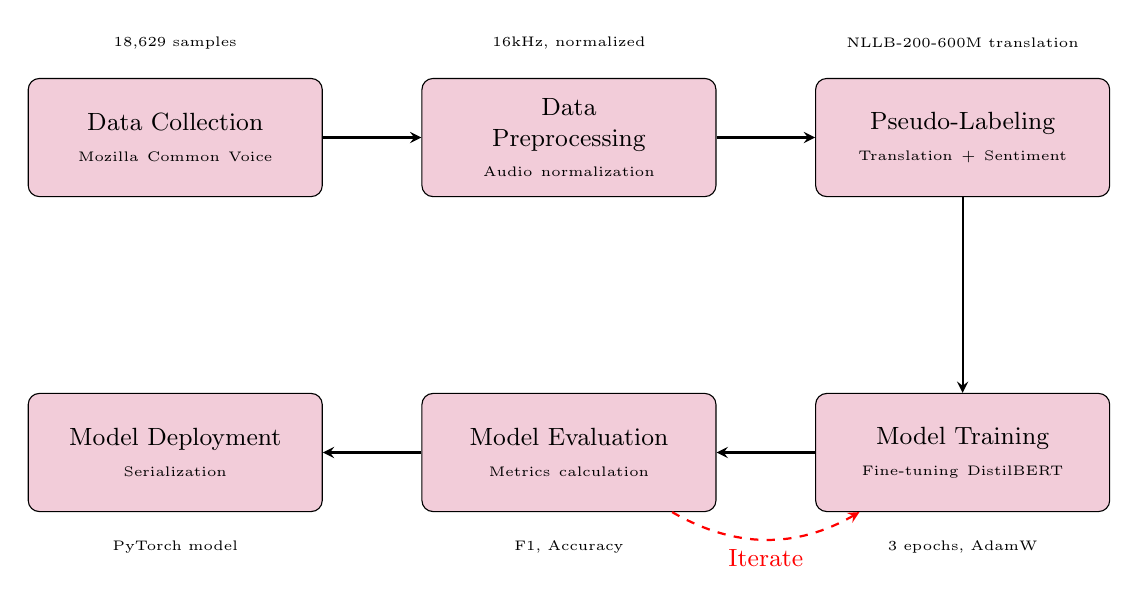
\begin{tikzpicture}[
    node distance=2.5cm,
    stage/.style={rectangle, draw, fill=purple!20, text width=3.5cm, text centered, rounded corners, minimum height=1.5cm, font=\small},
    arrow/.style={->, >=stealth, thick}
]

% Pipeline stages - arranged in two rows
\node[stage] (data) {Data Collection\\{\tiny Mozilla Common Voice}};
\node[stage, right of=data, xshift=2.5cm] (prep) {Data\\Preprocessing\\{\tiny Audio normalization}};
\node[stage, right of=prep, xshift=2.5cm] (label) {Pseudo-Labeling\\{\tiny Translation + Sentiment}};

\node[stage, below of=label, yshift=-1.5cm] (train) {Model Training\\{\tiny Fine-tuning DistilBERT}};
\node[stage, left of=train, xshift=-2.5cm] (eval) {Model Evaluation\\{\tiny Metrics calculation}};
\node[stage, left of=eval, xshift=-2.5cm] (deploy) {Model Deployment\\{\tiny Serialization}};

% Arrows
\draw[arrow] (data) -- (prep);
\draw[arrow] (prep) -- (label);
\draw[arrow] (label) -- (train);
\draw[arrow] (train) -- (eval);
\draw[arrow] (eval) -- (deploy);

% Feedback loop
\draw[arrow, dashed, red, thick] (eval) to[bend right=30] node[below, font=\small] {Iterate} (train);

% Annotations above
\node[above of=data, yshift=-1.3cm, text width=3.5cm, align=center, font=\tiny] {18,629 samples};
\node[above of=prep, yshift=-1.3cm, text width=3.5cm, align=center, font=\tiny] {16kHz, normalized};
\node[above of=label, yshift=-1.3cm, text width=3.5cm, align=center, font=\tiny] {NLLB-200-600M translation};

% Annotations below
\node[below of=train, yshift=1.3cm, text width=3.5cm, align=center, font=\tiny] {3 epochs, AdamW};
\node[below of=eval, yshift=1.3cm, text width=3.5cm, align=center, font=\tiny] {F1, Accuracy};
\node[below of=deploy, yshift=1.3cm, text width=3.5cm, align=center, font=\tiny] {PyTorch model};

\end{tikzpicture}
